\documentclass[twoside]{book}

% Packages required by doxygen
\usepackage{calc}
\usepackage{doxygen}
\usepackage{graphicx}
\usepackage[utf8]{inputenc}
\usepackage{makeidx}
\usepackage{multicol}
\usepackage{multirow}
\usepackage{fixltx2e}
\PassOptionsToPackage{warn}{textcomp}
\usepackage{textcomp}
\usepackage[nointegrals]{wasysym}
\usepackage[table]{xcolor}

% Font selection
\usepackage[T1]{fontenc}
\usepackage{mathptmx}
\usepackage[scaled=.90]{helvet}
\usepackage{courier}
\usepackage{amssymb}
\usepackage{sectsty}
\renewcommand{\familydefault}{\sfdefault}
\allsectionsfont{%
  \fontseries{bc}\selectfont%
  \color{darkgray}%
}
\renewcommand{\DoxyLabelFont}{%
  \fontseries{bc}\selectfont%
  \color{darkgray}%
}
\newcommand{\+}{\discretionary{\mbox{\scriptsize$\hookleftarrow$}}{}{}}

% Page & text layout
\usepackage{geometry}
\geometry{%
  a4paper,%
  top=2.5cm,%
  bottom=2.5cm,%
  left=2.5cm,%
  right=2.5cm%
}
\tolerance=750
\hfuzz=15pt
\hbadness=750
\setlength{\emergencystretch}{15pt}
\setlength{\parindent}{0cm}
\setlength{\parskip}{0.2cm}
\makeatletter
\renewcommand{\paragraph}{%
  \@startsection{paragraph}{4}{0ex}{-1.0ex}{1.0ex}{%
    \normalfont\normalsize\bfseries\SS@parafont%
  }%
}
\renewcommand{\subparagraph}{%
  \@startsection{subparagraph}{5}{0ex}{-1.0ex}{1.0ex}{%
    \normalfont\normalsize\bfseries\SS@subparafont%
  }%
}
\makeatother

% Headers & footers
\usepackage{fancyhdr}
\pagestyle{fancyplain}
\fancyhead[LE]{\fancyplain{}{\bfseries\thepage}}
\fancyhead[CE]{\fancyplain{}{}}
\fancyhead[RE]{\fancyplain{}{\bfseries\leftmark}}
\fancyhead[LO]{\fancyplain{}{\bfseries\rightmark}}
\fancyhead[CO]{\fancyplain{}{}}
\fancyhead[RO]{\fancyplain{}{\bfseries\thepage}}
\fancyfoot[LE]{\fancyplain{}{}}
\fancyfoot[CE]{\fancyplain{}{}}
\fancyfoot[RE]{\fancyplain{}{\bfseries\scriptsize Generated on Sat May 31 2014 00\+:46\+:02 for Lab 6 Factory by Doxygen }}
\fancyfoot[LO]{\fancyplain{}{\bfseries\scriptsize Generated on Sat May 31 2014 00\+:46\+:02 for Lab 6 Factory by Doxygen }}
\fancyfoot[CO]{\fancyplain{}{}}
\fancyfoot[RO]{\fancyplain{}{}}
\renewcommand{\footrulewidth}{0.4pt}
\renewcommand{\chaptermark}[1]{%
  \markboth{#1}{}%
}
\renewcommand{\sectionmark}[1]{%
  \markright{\thesection\ #1}%
}

% Indices & bibliography
\usepackage{natbib}
\usepackage[titles]{tocloft}
\setcounter{tocdepth}{3}
\setcounter{secnumdepth}{5}
\makeindex

% Hyperlinks (required, but should be loaded last)
\usepackage{ifpdf}
\ifpdf
  \usepackage[pdftex,pagebackref=true]{hyperref}
\else
  \usepackage[ps2pdf,pagebackref=true]{hyperref}
\fi
\hypersetup{%
  colorlinks=true,%
  linkcolor=blue,%
  citecolor=blue,%
  unicode%
}

% Custom commands
\newcommand{\clearemptydoublepage}{%
  \newpage{\pagestyle{empty}\cleardoublepage}%
}


%===== C O N T E N T S =====

\begin{document}

% Titlepage & ToC
\hypersetup{pageanchor=false,
             bookmarks=true,
             bookmarksnumbered=true,
             pdfencoding=unicode
            }
\pagenumbering{roman}
\begin{titlepage}
\vspace*{7cm}
\begin{center}%
{\Large Lab 6 Factory }\\
\vspace*{1cm}
{\large Generated by Doxygen 1.8.7}\\
\vspace*{0.5cm}
{\small Sat May 31 2014 00:46:02}\\
\end{center}
\end{titlepage}
\clearemptydoublepage
\tableofcontents
\clearemptydoublepage
\pagenumbering{arabic}
\hypersetup{pageanchor=true}

%--- Begin generated contents ---
\chapter{Hierarchical Index}
\section{Class Hierarchy}
This inheritance list is sorted roughly, but not completely, alphabetically\+:\begin{DoxyCompactList}
\item \contentsline{section}{Class\+\_\+\+A}{\pageref{class_class___a}}{}
\begin{DoxyCompactList}
\item \contentsline{section}{Class\+\_\+\+B}{\pageref{class_class___b}}{}
\item \contentsline{section}{Class\+\_\+\+C}{\pageref{class_class___c}}{}
\item \contentsline{section}{Class\+\_\+\+D}{\pageref{class_class___d}}{}
\end{DoxyCompactList}
\item \contentsline{section}{Factory}{\pageref{class_factory}}{}
\end{DoxyCompactList}

\chapter{Class Index}
\section{Class List}
Here are the classes, structs, unions and interfaces with brief descriptions\+:\begin{DoxyCompactList}
\item\contentsline{section}{\hyperlink{class_class___a}{Class\+\_\+\+A} }{\pageref{class_class___a}}{}
\item\contentsline{section}{\hyperlink{class_class___b}{Class\+\_\+\+B} }{\pageref{class_class___b}}{}
\item\contentsline{section}{\hyperlink{class_class___c}{Class\+\_\+\+C} }{\pageref{class_class___c}}{}
\item\contentsline{section}{\hyperlink{class_class___d}{Class\+\_\+\+D} }{\pageref{class_class___d}}{}
\item\contentsline{section}{\hyperlink{class_factory}{Factory} }{\pageref{class_factory}}{}
\end{DoxyCompactList}

\chapter{Class Documentation}
\hypertarget{class_class___a}{\section{Class\+\_\+\+A Class Reference}
\label{class_class___a}\index{Class\+\_\+\+A@{Class\+\_\+\+A}}
}
Inheritance diagram for Class\+\_\+\+A\+:\begin{figure}[H]
\begin{center}
\leavevmode
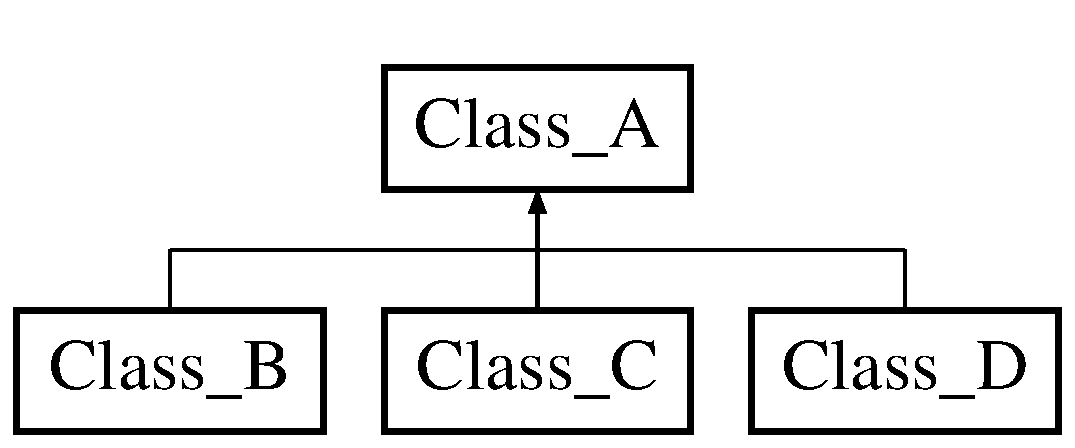
\includegraphics[height=2.000000cm]{class_class___a}
\end{center}
\end{figure}
\subsection*{Public Member Functions}
\begin{DoxyCompactItemize}
\item 
\hypertarget{class_class___a_a374f995672dfef87ae510b79424ed404}{virtual void \hyperlink{class_class___a_a374f995672dfef87ae510b79424ed404}{Show} (void)=0}\label{class_class___a_a374f995672dfef87ae510b79424ed404}

\begin{DoxyCompactList}\small\item\em Pure virtual method. \end{DoxyCompactList}\end{DoxyCompactItemize}


The documentation for this class was generated from the following files\+:\begin{DoxyCompactItemize}
\item 
Lab\+\_\+6\+\_\+\+Class\+\_\+\+Factory/Class\+\_\+\+A.\+h\item 
Lab\+\_\+6\+\_\+\+Class\+\_\+\+Factory/Class\+\_\+\+A.\+cpp\end{DoxyCompactItemize}

\hypertarget{class_class___b}{\section{Class\+\_\+\+B Class Reference}
\label{class_class___b}\index{Class\+\_\+\+B@{Class\+\_\+\+B}}
}
Inheritance diagram for Class\+\_\+\+B\+:\begin{figure}[H]
\begin{center}
\leavevmode
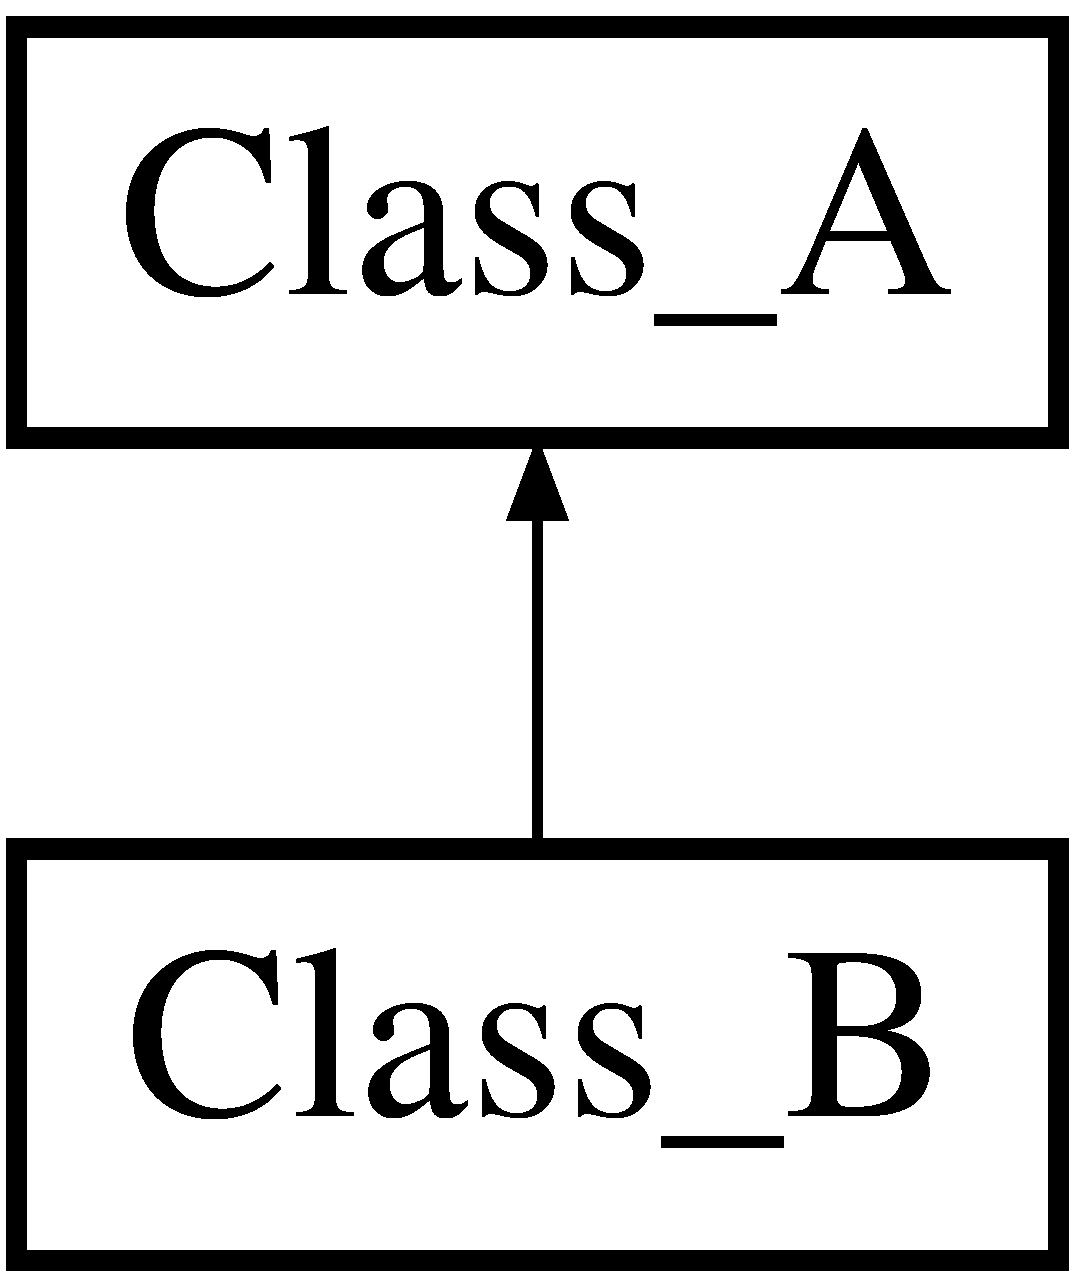
\includegraphics[height=2.000000cm]{class_class___b}
\end{center}
\end{figure}
\subsection*{Public Member Functions}
\begin{DoxyCompactItemize}
\item 
\hypertarget{class_class___b_a1d90a8dc22382d3b6fafe2cab30dd842}{void \hyperlink{class_class___b_a1d90a8dc22382d3b6fafe2cab30dd842}{Show} (void)}\label{class_class___b_a1d90a8dc22382d3b6fafe2cab30dd842}

\begin{DoxyCompactList}\small\item\em Print Class name. \end{DoxyCompactList}\end{DoxyCompactItemize}


\subsection{Detailed Description}
\hyperlink{class_class___a}{Class\+\_\+\+A} 

The documentation for this class was generated from the following files\+:\begin{DoxyCompactItemize}
\item 
Lab\+\_\+6\+\_\+\+Class\+\_\+\+Factory/Class\+\_\+\+B.\+h\item 
Lab\+\_\+6\+\_\+\+Class\+\_\+\+Factory/Class\+\_\+\+B.\+cpp\end{DoxyCompactItemize}

\hypertarget{class_class___c}{\section{Class\+\_\+\+C Class Reference}
\label{class_class___c}\index{Class\+\_\+\+C@{Class\+\_\+\+C}}
}
Inheritance diagram for Class\+\_\+\+C\+:\begin{figure}[H]
\begin{center}
\leavevmode
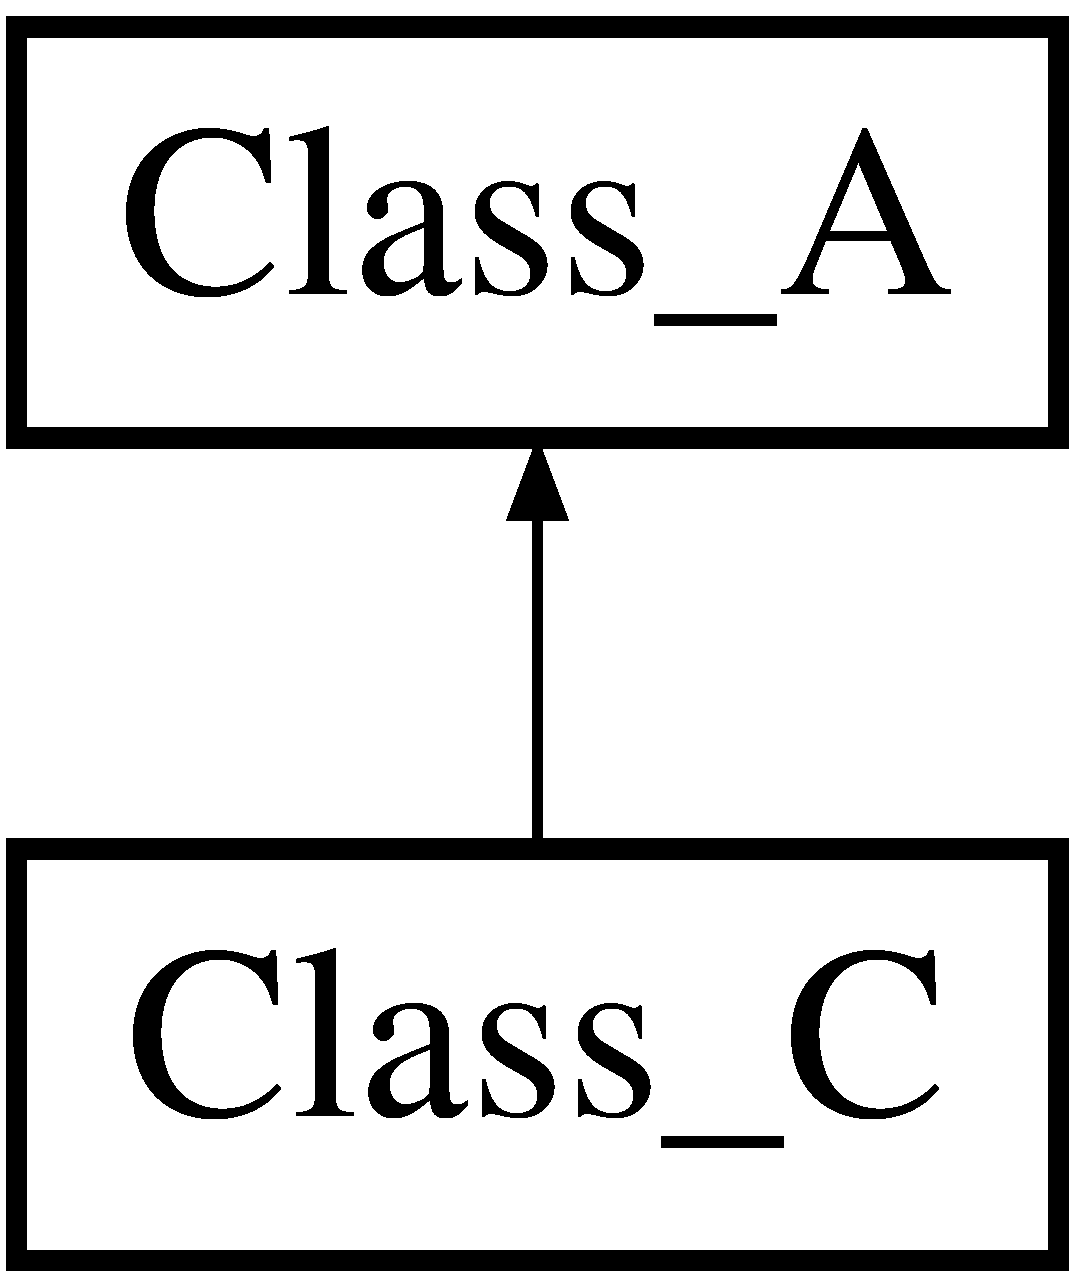
\includegraphics[height=2.000000cm]{class_class___c}
\end{center}
\end{figure}
\subsection*{Public Member Functions}
\begin{DoxyCompactItemize}
\item 
\hypertarget{class_class___c_abd1e1a1b11a87bb9c3dbe7fe208e4e63}{void \hyperlink{class_class___c_abd1e1a1b11a87bb9c3dbe7fe208e4e63}{Show} (void)}\label{class_class___c_abd1e1a1b11a87bb9c3dbe7fe208e4e63}

\begin{DoxyCompactList}\small\item\em Print Class name. \end{DoxyCompactList}\end{DoxyCompactItemize}


\subsection{Detailed Description}
\hyperlink{class_class___a}{Class\+\_\+\+A} 

The documentation for this class was generated from the following files\+:\begin{DoxyCompactItemize}
\item 
Lab\+\_\+6\+\_\+\+Class\+\_\+\+Factory/Class\+\_\+\+C.\+h\item 
Lab\+\_\+6\+\_\+\+Class\+\_\+\+Factory/Class\+\_\+\+C.\+cpp\end{DoxyCompactItemize}

\hypertarget{class_class___d}{\section{Class\+\_\+\+D Class Reference}
\label{class_class___d}\index{Class\+\_\+\+D@{Class\+\_\+\+D}}
}
Inheritance diagram for Class\+\_\+\+D\+:\begin{figure}[H]
\begin{center}
\leavevmode
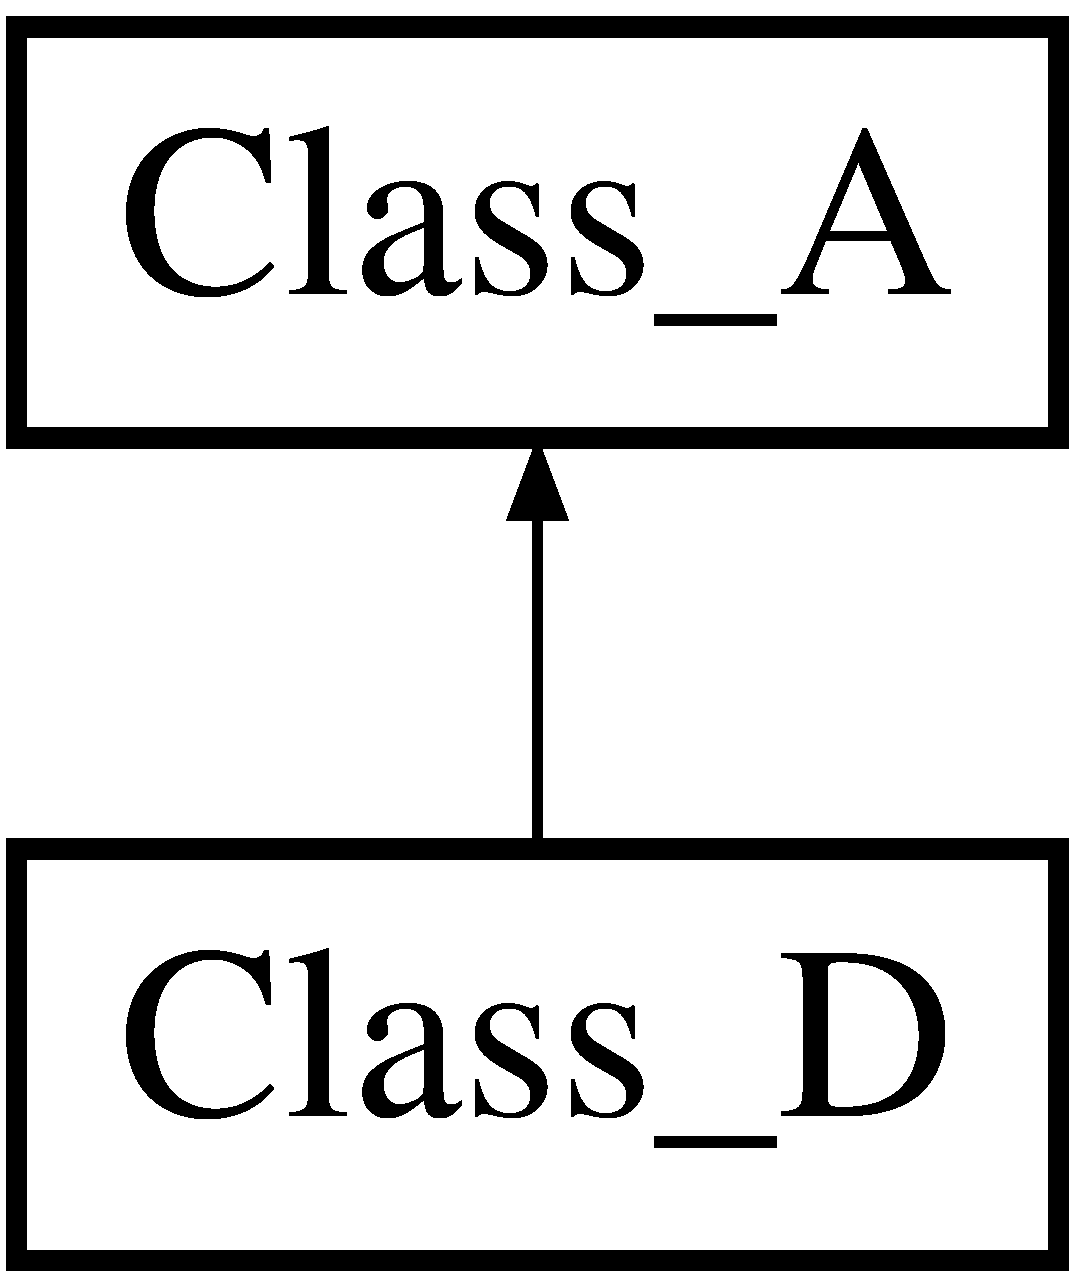
\includegraphics[height=2.000000cm]{class_class___d}
\end{center}
\end{figure}
\subsection*{Public Member Functions}
\begin{DoxyCompactItemize}
\item 
\hypertarget{class_class___d_ab98bb7922851ab7133863e6fb16aa17c}{void \hyperlink{class_class___d_ab98bb7922851ab7133863e6fb16aa17c}{Show} (void)}\label{class_class___d_ab98bb7922851ab7133863e6fb16aa17c}

\begin{DoxyCompactList}\small\item\em Print Class name. \end{DoxyCompactList}\end{DoxyCompactItemize}


\subsection{Detailed Description}
\hyperlink{class_class___a}{Class\+\_\+\+A} 

The documentation for this class was generated from the following files\+:\begin{DoxyCompactItemize}
\item 
Lab\+\_\+6\+\_\+\+Class\+\_\+\+Factory/Class\+\_\+\+D.\+h\item 
Lab\+\_\+6\+\_\+\+Class\+\_\+\+Factory/Class\+\_\+\+D.\+cpp\end{DoxyCompactItemize}

\hypertarget{class_factory}{\section{Factory Class Reference}
\label{class_factory}\index{Factory@{Factory}}
}
\subsection*{Public Member Functions}
\begin{DoxyCompactItemize}
\item 
\hyperlink{class_class___a}{Class\+\_\+\+A} $\ast$ \hyperlink{class_factory_ae0c1e6992f57e1c0eac8e3d155f57c28}{Create} (int I\+D)
\end{DoxyCompactItemize}


\subsection{Member Function Documentation}
\hypertarget{class_factory_ae0c1e6992f57e1c0eac8e3d155f57c28}{\index{Factory@{Factory}!Create@{Create}}
\index{Create@{Create}!Factory@{Factory}}
\subsubsection[{Create}]{\setlength{\rightskip}{0pt plus 5cm}{\bf Class\+\_\+\+A} $\ast$ Factory\+::\+Create (
\begin{DoxyParamCaption}
\item[{int}]{I\+D}
\end{DoxyParamCaption}
)}}\label{class_factory_ae0c1e6992f57e1c0eac8e3d155f57c28}
Create pointer to class B, C or D 
\begin{DoxyParams}{Parameters}
{\em I\+D} & of created object's class I\+D = 1 =$>$ Class B I\+D = 3 =$>$ Class C I\+D = 3 =$>$ Class D \\
\hline
\end{DoxyParams}


The documentation for this class was generated from the following files\+:\begin{DoxyCompactItemize}
\item 
Lab\+\_\+6\+\_\+\+Class\+\_\+\+Factory/Factory.\+h\item 
Lab\+\_\+6\+\_\+\+Class\+\_\+\+Factory/Factory.\+cpp\end{DoxyCompactItemize}

%--- End generated contents ---

% Index
\newpage
\phantomsection
\addcontentsline{toc}{chapter}{Index}
\printindex

\end{document}
